\documentclass[../piano-di-progetto.tex]{subfiles}
\begin{document}

\subsection{Verifica e collaudo}
Questo macro periodo inizia il 2020-06-11, dopo la consegna dei documenti, e termina il giorno 2020-07-20 con la consegna per la revisione di accettazione. Verranno svolti due incrementi.

\subsubsection{Ruoli}
Durante questa macro, viene richiesta la presenza dei seguenti ruoli:
\begin{itemize}
    \item Responsabile;
    \item Amministratore;
    \item Progettista;
    \item Programmatore;
    \item Verificatore.
\end{itemize}

\subsubsection{X incremento}
 Vengono stabiliti i seguenti obiettivi per il decimo incremento:
 \begin{itemize}
     \item Revisione e aggiornamento dei documenti;
     \item Codifica dei test.
 \end{itemize}

\paragraph{Attività}
Le attività verranno svolte in un unico periodo:
\\
\\
\textbf{Periodo unico(2020-06-18 - 2020-06-28)}
\begin{itemize}
        \item \textbf{Normazione}: revisione e aggiornamento delle norme;
        \item \textbf{Pianificazione}: revisione e aggiornamento della pianificazione;
        \item \textbf{Qualità}: revisione e aggiornamento della pianificazione di qualità;
        \item \textbf{Codifica dei test};
        \item \textbf{Verifica}.
\end{itemize}

\subsubsection{XI incremento}
 Vengono stabiliti i seguenti obiettivi per l'undicesimo incremento:
 \begin{itemize}
     \item Scrittura finale dei documenti;
     \item Rilascio ultima versione;
     \item Verifica e collaudo.
 \end{itemize}

\paragraph{Attività}
Le attività verranno svolte in un unico periodo:
\\
\\
\textbf{Periodo unico (2020-06-29 - 2020-07-12)}:
\begin{itemize}
    \item \textbf{Codifica}: rilascio della versione finale;
    \item \textbf{Stesura finale del manuale};
    \item \textbf{Stesura finale del consuntivo};
    \item \textbf{Verifica e collaudo finale}.
\end{itemize}



\newpage
\begin{landscape}
    \begin{figure}[H]
        \centering
        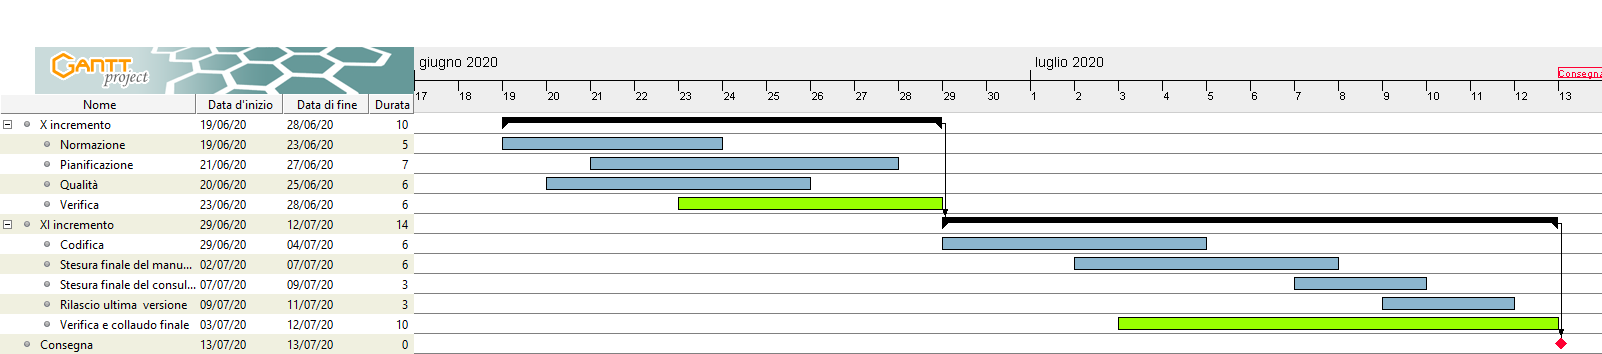
\includegraphics[width=24cm]{img/verifica.png}
        \caption{Diagramma attività nel periodo di verifica e collaudo}
      \end{figure}
\end{landscape}


\end{document}
